\chapter{Text recognition algorithms}

Text recognition forms the basis of any complex OCR software. Its task is to transform an input image into its segmented form, with segments containing information about individual characters and their positions.

We begin this chapter by presenting various aspects that impact the quality of the input image, which we have observed to affect the results of the text recognition algorithms. To reduce the effects of these aspects, we also focus on the related task of preprocessing the input image. After that, we analyze the individual steps of the text detection process and review the existing techniques used for this purpose.
	
\section{Common obstacles of successful text recognition}

Even for human perception, the task of recognizing text in a complex document might become difficult due to various factors. Text recognition engines work similarly or, in some specific cases trivial for human perception, even worse.

Common difficulties faced by text recognition algorithms have been reviewed by~\citet{preprocessAll}. These can be categorized into following major classes:

\begin{description}

\item[Font face variability] Text documents contain a lot of different fonts and styles, including different headings, body text, footer and header sizes along with bold, italics and underlined characters, differently colored fonts and even custom-made fonts. Furthermore, when it comes to handwritten text, each character is slightly different and the text contains a lot of inaccuracies. To hold the information about every possible font and style would therefore be impractical for any OCR software, and, in case of custom-made fonts or handwritten text, even impossible. Therefore, an OCR software needs to use heuristics to match the actual symbol it recognized to its expectation of the character shape. This does not always produce the desirable results. In specific cases, especially in decorative fonts or handwritten text, characters like S or 5, 0 or O and I or l are hard to distinguish even by human perception. This often results in the failure of text detection algorithm for these specific characters.

\item[Scan quality] The optimal results of image acquisition techniques, like scanning, are high-contrast images with no inaccuracies. However, the scanning process often disrupts the input image, which results in low contrast, insufficient sharpness, pixelation, noise and disruption of lines. This is usually due to a low resolution scan or human made mistakes during scanning. We use the techniques of preprocessing to try and reconstruct this error prone image into a suitable input for text recognition engines.

\item[Skew problems] Photographing or scanning an image often results in minor human made skew and rotation inaccuracies. However, most of the text recognition engines already assume the input to be properly vertically and horizontally aligned for the simplicity and lower time complexity of its algorithm. This causes the engines to fail on skewed images. Therefore, we attempt to deskew the input images during preprocessing with the use of deskewing techniques.

\item[Colors] To distinguish characters from the image background, OCR engines use various techniques based on the color values of the individual pixels, their contrast, brightness, etc. When it comes to monochrome one images, to determine this division of image pixels is a simple task. With colored inputs, however, many complications arise. For example, recognition of green text on a red background fails when presented to a method based on contrast. This and improved time complexity of the algorithm is the reason why images often undergo the process of binarization. 

\end{description}

These difficulties motivate the common OCR implementations to work with optimistic assumptions about documents, such as that the document has only one column, that it is not handwritten, and that its lines are horizontally aligned.

Several existing image processing techniques may be used to eliminate the effects of most of these obstacles in the attempt to increase the performance of OCR engines. We review the most important of them in the next section.

\section{Preprocessing for OCR}

Many of the existing OCR engines are equipped with several simple built-in preprocessing methods. It is, however, often beneficial to preprocess the image using specialized tools in order to obtain better input for the OCR. In this section, we discuss the most effective and commonly used image transformations for that purpose.

\subsection{Scaling} \label{scaling}

In computer graphics, scaling refers to the process of changing the resolution of a digital image while preserving its data content. In OCR, the purpose of this method is to provide an input of viable size for existing OCR engines. For example, OCR engines likes Tesseract~\cite{TesseractQual} or ABBYY FineReader~\cite{ABBYYdpi} encourage their users to use 300 dpi images --- this is due to the fact that the classification of newly recognized characters requires a large set of training data which they are then compared to; which are, in this case, most often obtained from 300 dpi images. 300 dpi is claimed to be high enough resolution for a clear recognition of character features in common text, but also low enough to maintain a reasonable execution time of the algorithm.

If the user has provided us with an image of a different resolution, the image therefore needs to be either upscaled (if the dpi of the input image was lower) or downscaled (if the dpi of the input image was higher). For these purposes, interpolation-based algorithms are used.

Interpolation attempts to minimize the aliasing effect of the resulting image, so the scaled picture does not appear visibly pixelated and its edges are not jagged. It is based on using known data to estimate values at unknown points. It specifically approximates the color and intensity of the resulting pixel based on the values at surrounding pixels. When downscaling, this technique therefore computes one color value for each set of pixels, which are the color values of the pixels in the new image. When upscaling, it computes color values of the new pixels by approximating the values of the old pixels around them.

Existing interpolation algorithms can be grouped into two categories: adaptive and non-adaptive.

Adaptive methods change the way they treat various pixels depending on whether are they a part of a smooth texture or a sharp edge. They are primarily designed to minimize the presence of interpolation artifacts in regions where they are most apparent. Examples of adaptive methods include e.g. Spline, Sinc, Lanczos or Discrete Wavelet Transforms~\cite{interpolation}.

Non-adaptive methods, on the other hand, treat all pixels equally. Their complexity and classification depends on the size of pixel neighborhood they interpolate~\cite{interpolation}. The effects of several of these methods are detailed in~\cref{fig:preprocessInterpolation}.

\begin{figure}[t]
\centering
{\sffamily
\begin{tabular}{ccc}
& Original & \\
&
\includegraphics{img/preprocessing/interp_original.png}&\\
\vspace{1em} \\
Nearest-neighbor& Bilinear interpolation & Bicubic interpolation \\
interpolation &&\\

\includegraphics[width=.3\linewidth]{img/preprocessing/interp_nearestNeighbor.png}
&

\includegraphics[width=.3\linewidth]{img/preprocessing/interp_bilinear.png}
&

\includegraphics[width=.3\linewidth]{img/preprocessing/interp_bicubic.png}
\end{tabular}
}
\caption{Comparison of results of several non-adaptive interpolation methods, scaled $4{\times}$ (image by~\citet{nonAdaptiveInterp}).}
\label{fig:preprocessInterpolation}
\end{figure}

Although the results of adaptive methods are more accurate, they are not generally for OCR preprocessing due to their high time complexity. Therefore, the most popular decision for general cases is the use of Bicubic interpolation method~\cite{interpolationComp}.

\subsection{Contrast enhancement} \label{contrastEnhancemet}

Contrast is the difference in luminance or colour that makes objects in the same field of view distinguishable. Low contrast often results in blending of edges during recognition, which decreases the accuracy of OCR.

An image histogram is used to improve this aspect. A histogram is a representation of the distribution of data and, in case of image histograms, it represents the tonal distribution of an image --- x-axis stands for all available tonal levels, and y-axis represents the number of pixels for each tonal level. In colored (RGB) images, the histogram is represented by three separate histograms, one for each color component. By spreading out the most frequent intensity values in the histogram, as shown in~\cref{fig:preprocessContrastComparison}, the contrast of the image increases.

\begin{figure}[t]
\centering
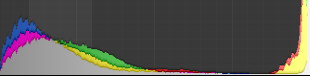
\includegraphics[width=0.4\linewidth]{img/preprocessing//histogram_low.png}
\qquad
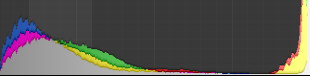
\includegraphics[width=0.4\linewidth]{img/preprocessing/histogram_high.png}
\caption{Histogram-based comparison of image contrast. Left: low-contrast image histogram, right: high-contrast image histogram.}
\label{fig:preprocessContrastComparison}
\end{figure}

Histogram stretching methods are categorized as methods of\emph{linear stretching} and \emph{non-linear stretching}~\citep{linearNonStretch}, depending on the forms of functions they use. Although linear methods are easier to implement and do not cause the objects in the original image to lose their brightness values, non-linear methods were shown to produce better results in general case~\citep{chandpa1comparative}. Despite of that, linear methods still deliver satisfactory results on images with Gaussian or near-Gaussian histograms.

The most popular choice for contrast enhancement for OCR is a non-linear technique called \emph{histogram equalization}~\citep{histogramEQ}. Although it produces unrealistic and over-enhanced effects in photographs, the over-processing actually suits the text data. The typical output of histogram equalization on textual data is displayed in~\cref{fig:preprocessHistogramEqualization}.

\citet{contrastOther} describe other methods of contrast enhancement, like CLAHE, Dynamic Stochastic Resonance and generic transforms, such as Fourier, Discrete Cosine, and Wavelet. For complex text recognition cases, CLAHE method can be used with satisfactory results.

\begin{figure}[t]
\centering
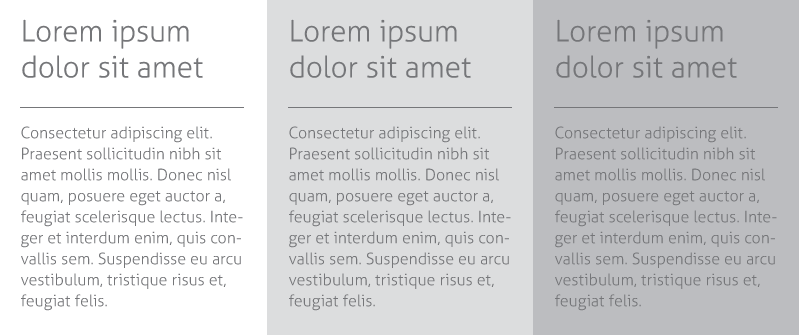
\includegraphics[width=0.4\linewidth]{img/preprocessing/contrast_low.png}
\qquad
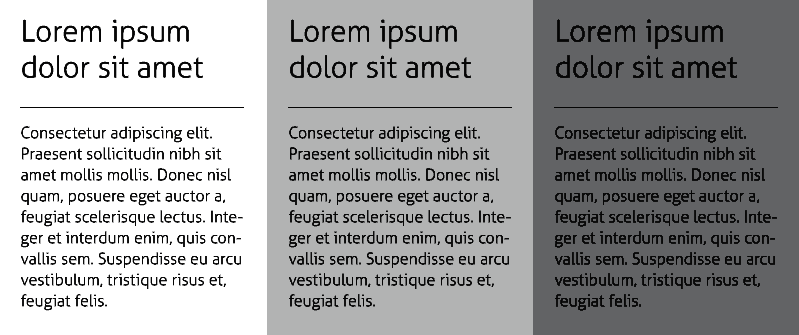
\includegraphics[width=0.4\linewidth]{img/preprocessing/contrast_high.png}
\caption{Results of histogram-based equalization. Left: original image, right: processed image.}
\label{fig:preprocessHistogramEqualization}
\end{figure}

\subsection{Binarization} \label{binarization}

To recognize characters in an image, an OCR software must distinguish the background pixels from the actual pixels that belong to the characters. To determine the boundaries between these two groups in a colored image is a complex task due to the need of processing the whole RGB information of each pixel. However, there might be a loss of information when converting an RGB image to grayscale/monochrome. Therefore, the approach to the conversion can not be naive and must consider unusually colored images (e.g. green fonts on a red background).

\subsubsection{Grayscale conversion} \label{grayscaleConversion}

Grayscale conversion is the process of assigning each pixel of an image a gray value, while preserving as much information of the original image as possible. The simplest approach to grayscale conversion is the averaging approach, which assigns each pixel the average of its R, G and B value. However, this approach causes the blending of colors of similar luminance contrast (such as the already mentioned greens and reds). Additionally, human perception of colors is non-uniform --- green color is perceived more strongly than red, and red more strongly than blue. For these reasons, a correction formula (often called \emph{luma}~\cite{grayscaleConv}) that weights each color component differently is used. Slight differences in the results of these techniques are demonstrated in~\cref{fig:preprocessGrayscale}.

Other more complicated methods were reviewed by~\citet{grayscaleCadik}.

\begin{figure}[t]
\centering
{\sffamily
\begin{tabular}{ccc}
Original & Averaging technique & Luma correction \\
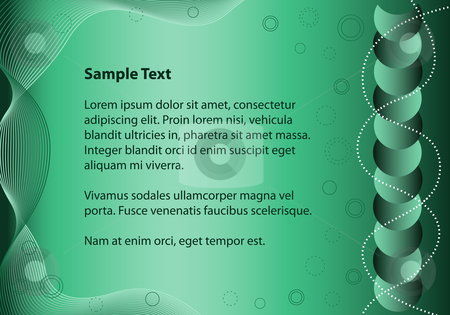
\includegraphics[width=.28\linewidth]{img/preprocessing/grayscale_orig.jpg}
&
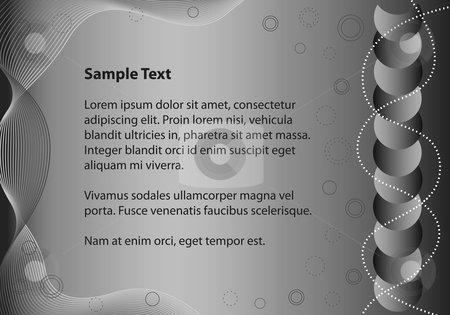
\includegraphics[width=.28\linewidth]{img/preprocessing/grayscale_avg.png}
&
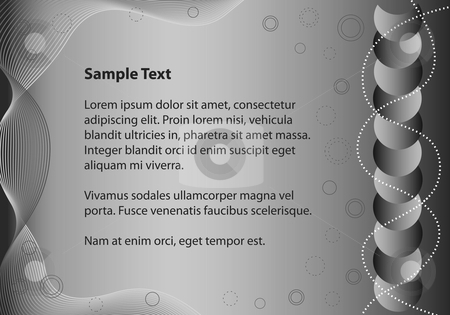
\includegraphics[width=.28\linewidth]{img/preprocessing/grayscale_luma.png}
\end{tabular}
}
\caption{Comparison of grayscale techniques.}
\label{fig:preprocessGrayscale}
\end{figure}

\subsubsection{Threshold-based binarization}

Binarization of an image is usually performed on grayscale images, which we obtain from a colored input by previously mentioned techniques. Most of the binarization methods work on the basis of a \emph{threshold} --- a value that determines whether the pixel should be black or white in the resulting binarized image. Various binarization methods differ in the way that this threshold is calculated and used.

\emph{Global thresholding}~\citep{globalThresh} is the simplest approach to binarization. It works by choosing a threshold value and iterating over the whole image, comparing the value of each pixel to this threshold. However, as the brightness and contrast of different images vary, it is generally impossible to choose a threshold suitable for all images.

More complex methods that aim to correct the problems of global thresholding exist. Some of these include:
\begin{itemize}
\item Otsu's method for global threshold estimation~\citep{otsu}
\item Local-thresholding methods~\citep{localOtherBin}:
\begin{itemize}
\item Niblack method
\item Bernsen method
\item Sauvola method
\end{itemize}
\end{itemize}

Otsu's method statistically computes a global threshold by a dynamical classification of image pixels into background and foreground pixels. Although simple and easy to implement, but, as any global method, it is inherently unable to fix high variance or uneven spots in an image background. Local-thresholding methods aim to solve this issue by allowing different threshold values in different parts of the image. They differ in the way the existing thresholds are computed --- for example, Niblack's method~\citep{adaptiveBin} uses mean and standard deviation of surrounding pixels for each pixel, Sauvola method improves it by checking for blank regions and Bernsen's method by optimizing Niblack's computations. 

Visual differences between the mentioned methods are displayed in~\cref{fig:preprocessBinarization}. Comprehensive reviews of other, more complex methods are also available~\citep{localOtherBin}.

\begin{figure}
\centering
{\sffamily
\begin{tabular}{ccc}
Original scanned image &
Global Thresholding &
Sauvola Binarization \\
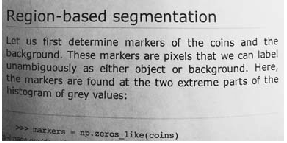
\includegraphics[width=.3\linewidth]{img/preprocessing/bin_orig.png} &
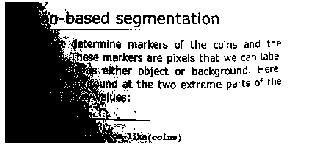
\includegraphics[width=.3\linewidth]{img/preprocessing/bin_glob.png} &
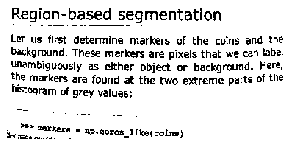
\includegraphics[width=.3\linewidth]{img/preprocessing/bin_sauvola.png}
\end{tabular}
}
\caption{Comparison of binarization method output on an unevenly lit image. Images demonstrated by~\citet{binarizationComp}.}
\label{fig:preprocessBinarization}
\end{figure}

\subsection{Deskewing} \label{deskewing}

Skewed images are probably the most common problem that many OCR engines struggle with. They usually appear when an image is scanned or photographed from an angle.

Negative effects of skewed images are most apparent in results of page segmentation (see~\cref{pageSegmentation}), as this process often relies on the characters to be properly vertically and horizontally aligned.

In this section, we present various methods of image deskewing. All of them work (for more accurate results) after binarization of the image and generally assume the skew angle to be no more than $20^{\circ}$. Although algorithms that work on greater skew angles also exist~\citep{skewAngleDetection}, they are not as widely used for the purposes of deskewing scanned documents, which are generally only slightly tweaked.

The most effective and popular algorithms include the following~\citep{skewBestTechniques}:
\begin{itemize}
    \item Hough transform~\cite{houghTransform}
    \item Projection profile method~\cite{skewAngleDetection}
    \item Cross correlation~\cite{skewAngleDetection}
    \item Connected component clustering (or nearest-neighbor clustering)~\citep{skewClustering}
\end{itemize}

Hough transform applies feature extraction to the image, takes the line with the highest pixel count, and computes the skew of the whole document using this line. Projection profile method rotates the image multiple times and computes the histogram along horizontal scan lines. The skew of the rotated image where the histogram has the most peaks and valleys is determined to be the skew of the input image. Cross correlation method is based on applying the projection profile method to multiple vertical segments, and Connected component clustering method is based on finding the coherency between connected components of the image and determining their common skew. We present the overview and comparison of these methods in~\cref{tab:preprocessSkewProsCons}.

Other methods of deskewing may also be used. These include Fourier~\citep{fourierTransform}, Wavelet Decomposition, Radon Transform, PCP, one-pass or multi-pass skew correction, morphology algorithms, etc.

\begin{table}[t]
\renewcommand{\arraystretch}{1.5}
{\footnotesize
\begin{tabular}{p{8em}p{7em}p{2.5em}p{6em}p{9em}}
\toprule
\textbf{Method} & \textbf{Performance} & \textbf{Max. skew} & \textbf{Image handling} & \textbf{Setbacks} \\
\midrule
Hough transform
&
slow
&
$90^{\circ}$
&
sufficient
&
--
\\
Projection profiles
&
slow
&
$10^{\circ}$
&
problematic
&
--
\\
Cross correlation
&
relatively fast
&
$10^{\circ}$
&
problematic
&
works only on simple documents
\\
Connected component clustering
&
clustering-dependent
&
$20^{\circ}$
&
good
&
requires high-quality input
\\
\bottomrule
\end{tabular}
}
\caption{The advantages and disadvantages of different deskewing methods.}
\label{tab:preprocessSkewProsCons}
\end{table}

\begin{figure}
\centering
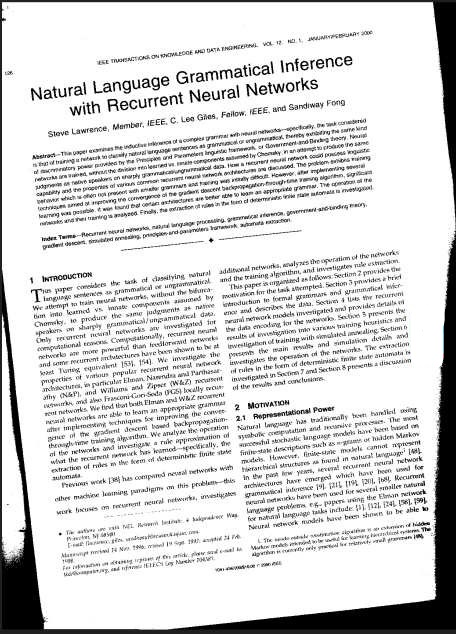
\includegraphics[height=0.25\textheight]{img/preprocessing/deskew_orig.jpg}
\qquad
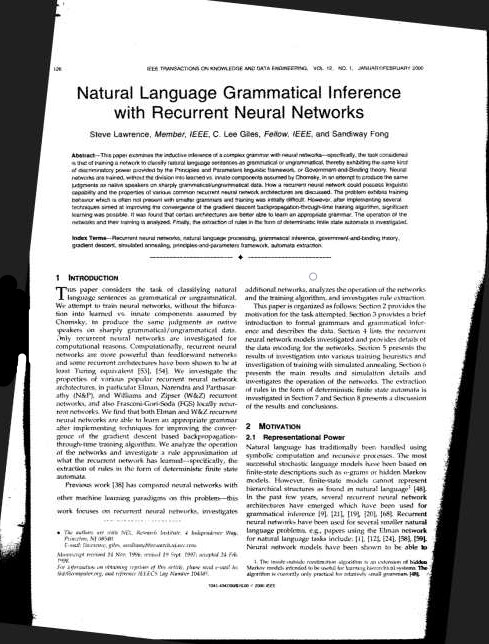
\includegraphics[height=0.25\textheight]{img/preprocessing/deskew_new.jpg}
\caption{Image deskewing illustrated. Left: original image, right: deskewed image.}
\label{fig:preprocessDeskewing}
\end{figure}

\subsection{Noise reduction}

Image noise is an usually unwanted random variation of brightness or color information in images, similar to film grain in digital cameras. It is often caused by the inevitable physical variance in amount of light recorded by a scanner or a digital camera.

The presence of noise negatively affects the quality of the image by e.g. disrupting sharp edges of elements. This causes the process of specific OCR steps, such as edge detection, to output less accurate data, which can lead to the failure of character recognition.

Common image processing filters are used~\citep{denoisingTechniques} when performing noise reduction. These can be categorized as either linear or non-linear, depending on their linearity relationships.

\begin{figure}[t]
\centering
{\sffamily
\begin{tabular}{cc}
Original & Gaussian filter \\
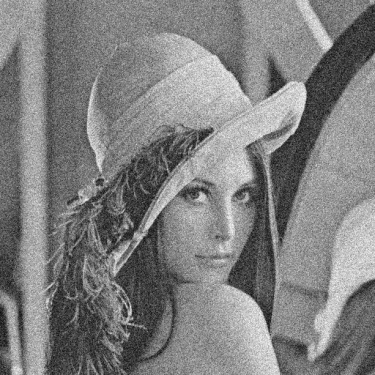
\includegraphics[width=.4\linewidth]{img/preprocessing/denoise_orig.png}
&
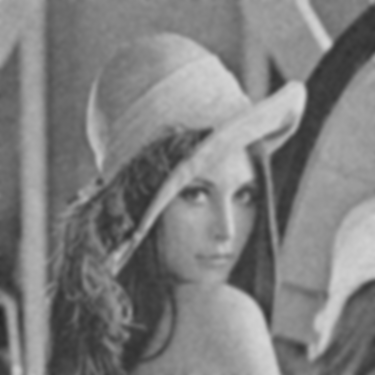
\includegraphics[width=.4\linewidth]{img/preprocessing/denoise_gauss.png}
\vspace{1em} \\
Median filter & Non-local means method \\
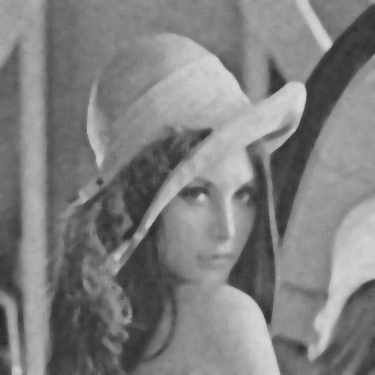
\includegraphics[width=.4\linewidth]{img/preprocessing/denoise_median.png}
&
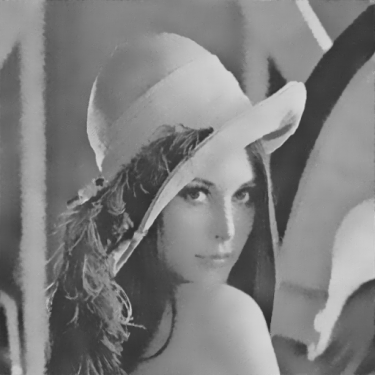
\includegraphics[width=.4\linewidth]{img/preprocessing/denoise_nonlocal.png}
\end{tabular}
}
\caption{Comparison of denoising techniques.}
\label{fig:preprocessDenoising}
\end{figure}

\emph{Linear filtering}, such as mean filtering, Gaussian filtering or Wiener filtering, processes each pixel by linearly combining the values of its neighborhood pixels. This, however, often results in blurred edges and smoother fine details. As these methods require only a small amount of computations (which leads to increased speed and simple implementation), they are still widely used.

\emph{Non-linear filtering}, on the other hand, renders an output which is not a linear function of its input. Methods based on non-linear filtering used for denoising purposes include filters like \emph{median filter}, which computes the value of the resulting pixel from a local median, or \emph{non-local means method}~\citep{nonLocalMeans}, which is based on taking a mean value of all pixels in the image weighted by their similarity to the target pixel. Both methods produce sharper and clearer images than linear filters at the expense of increased run time.

We provide a comparison of the above mentioned methods in~\cref{fig:preprocessDenoising}.

\subsection{Scanning border reduction}

Scanned documents often have visible dark borders (\emph{marginal noise}). These originate either during scanning (due to the presence of neighbouring pages) or are an unwanted result of the binarization process (see~\cref{binarization}). 

Marginal noise can cause negative effects on the results of OCR, as it may either be interpreted as a part of character symbols due to its structure, or it may interfere with other page elements.

Algorithms focusing on marginal noise reduction often perceive it as a dark connected component of the page. Therefore, they use connected component extraction to recognize and further remove these components. An example of a connected component based scanning border reduction algorithm was presented by~\citet{marginalNoiseWindow}.

Another slightly different approach was described by~\citet{marginalNoiseEdge}. It is based on edge density calculations, and the fact that text areas have generally a much lower density than edge areas. This approach uses an edge detector to examine the presence of both vertical and horizontal noise. Its removal is the performed by by filters or other heuristic algorithms.

We demonstrate the effects of scanning border reduction in~\cref{fig:marginalNoise}.

\begin{figure}
\centering
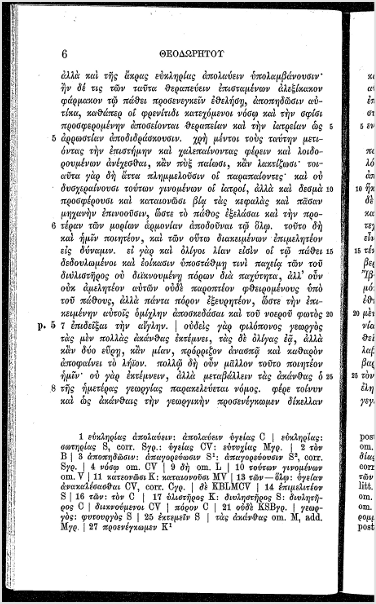
\includegraphics[height=10em]{img/preprocessing/scan_borders_orig.png}
\qquad
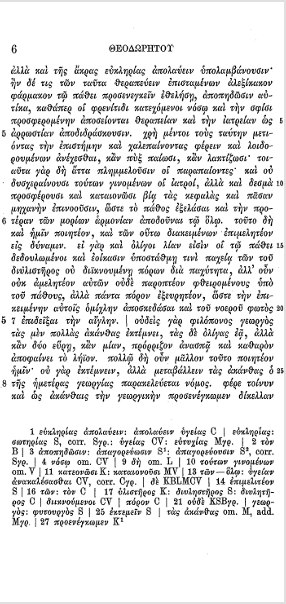
\includegraphics[height=10em]{img/preprocessing/scan_borders_result.png}
\caption{Removal of scanning artifacts, as presented by~\citet{TesseractQual}. Left: original, right: removed scanning borders.}
\label{fig:marginalNoise}
\end{figure}

\section{Text detection process}

The goal of text detection is to recognize and classify individual textual elements of an image document and interpret them as textual contents of the document.

There exist two main approaches for text detection in OCR:
\begin{enumerate}
    \item heuristic-based approaches
    \item neural-network-based approaches
\end{enumerate}

In this paper, we concentrate on the heuristic-based approach of the OCR problem, as we use it in our implementation. However, neural network recognition is a promising field of study and also deserves a mention.

Although OCR engines greatly differ in the way their heuristic approaches work, they generally contain the following steps:
\begin{enumerate}
    \item \emph{Page segmentation} --- logical and topological division of the page into multiple smaller segments.
    \item \emph{Feature extraction} --- simplification of the extracted elements of the image to small, informative inputs viable for standalone recognition.
    \item \emph{Character classification}
\end{enumerate}

We analyze these steps in the individual subsections below.

\subsection{Page segmentation} \label{pageSegmentation}

The task of page segmentation is to extract page sections that contain uniformly-formatted bodies of characters (e.g.~columns or paragraphs) that can be easily passed to later steps of text recognition.

Page segmentation can be performed in three different ways~\citep{segmentationOverview} --- either we start with an image as a whole and recursively divide it into parts until certain criterion is met (top-down), or we start with individual pixels and group them according to similarity of their attributes (bottom-up), or we use a combination of these two methods.

In this section, we focus mostly on a method used by the Tesseract engine~\cite{tesseractSegmentationTab}. For comparison, we also overview several other existing techniques.

\subsubsection{Tesseract page segmentation} \label{sectionTessPageSegm}

In this section, we are concerned with a page segmentation technique proposed by~\citet{tesseractSegmentationTab}. This method is based on detecting tab-stops.

Tab-stops are used in word processors to enable obvious alignment of text, and are present in documents as margins, column edges, or indentations. All of them are placed at fixed x-positions, at which edges or centers of text lines are vertically aligned.

Following are the individual steps of the tab-stop based page segmentation algorithm (\cref{fig:segmentationTesseract1}):
\begin{enumerate}
    \item Obtain the input image document (\cref{fig:segmentationTesseract1}).
    \item Find the connected components of the document image.
    \item Select candidate tab-stop components from connected components by analyzing their alignment.
    \item Group the discovered candidate tab-stop components into vertical lines (\cref{fig:segmentationTesseract2}).
    \item Create tab-lines by examining the alignment of the vertical lines.
    \item Create \emph{column partitions} from the connected components of the layout analysis so they do not cross any tab-lines and are of the same type (e.g. text, image, form) (\cref{fig:segmentationTesseract3}).
    \item Merge column partitions into columns (\cref{fig:segmentationTesseract4}).
    \item Based on the positioning of columns and heuristics (different types of fonts, line spacing), merge or divide existing column partitions into segmented blocks. (\cref{fig:segmentationTesseract5}).
\end{enumerate}

\begin{figure}[p]
\centering
\begin{subfigure}{0.30\textwidth}
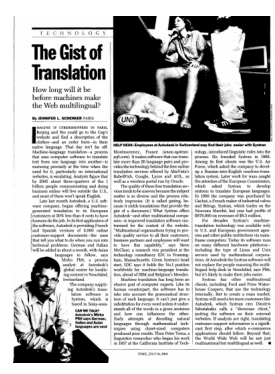
\includegraphics[width=\linewidth]{img/tabStopDetection/tessPageSegm1.png}
\caption{The original input image.}
\label{fig:segmentationTesseract1}
\end{subfigure}
\quad
\begin{subfigure}{0.30\textwidth}
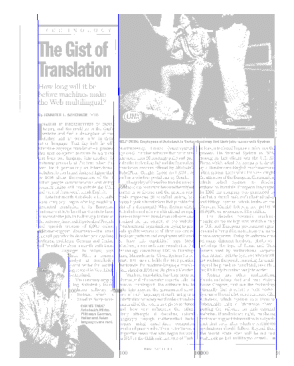
\includegraphics[width=\linewidth]{img/tabStopDetection/tessPageSegm2.png}
\caption{Connected components grouped into vertical lines. Upon close inspection, we can see that each page column has multiple groups of connected components.}
\label{fig:segmentationTesseract2}
\end{subfigure}
\quad
\begin{subfigure}{0.30\textwidth}
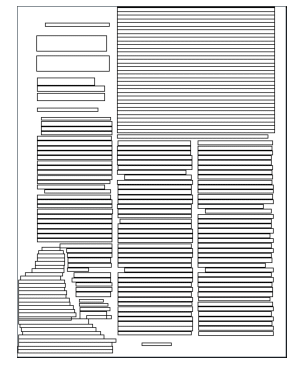
\includegraphics[width=\linewidth]{img/tabStopDetection/tessPageSegm3.png}
\caption{Column partitions created from connected components and individual tab-lines.}
\label{fig:segmentationTesseract3}
\end{subfigure}
\\
\begin{subfigure}{0.30\textwidth}
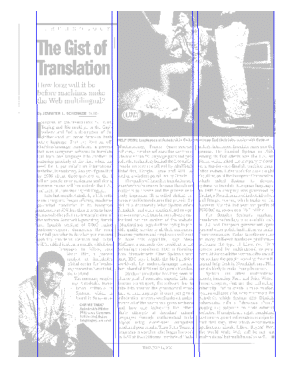
\includegraphics[width=\linewidth]{img/tabStopDetection/tessPageSegm4.png}
\caption{Column partitions merged into columns. Upon close inspection, we can see that the recognized columns are almost identical to the actual page columns.}
\label{fig:segmentationTesseract4}
\end{subfigure}
\quad
\begin{subfigure}{0.30\textwidth}
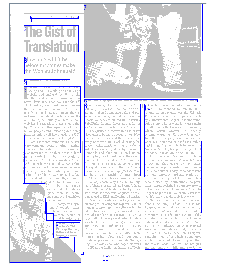
\includegraphics[width=\linewidth]{img/tabStopDetection/tessPageSegm5.pdf}
\caption{The final segmented blocks.}
\label{fig:segmentationTesseract5}
\end{subfigure}
\caption{The process of Tesseract table recognition~\cite{tesseractSegmentationTab}.}
\label{fig:segmentationTesseract}
\end{figure}

This method is implemented and used by the Tesseract engine with the preprocessing help of the Leptonica library. It claims to yield satisfactory results, given the input document is properly preprocessed.

\subsubsection{Other page segmentation techniques}

In this section, we briefly overview the principles of the most popular page segmentation techniques, already described by~\citet{segmentationOverview}, such as RXYC algorithm, Smearing algorithm, Voronoi diagram based algorithm, Docstrum algorithm, Whitespace analysis and Contrained text-line detection. Their core ideas greatly differ and therefore, their behaviours vary depending on the input.

For example, RXYC algorithm perceives the input page as a tree and recursively splits its nodes, dividing the page into smaller segments. Smearing algorithm, on the other hand, is a bottom-up approach based on linking black areas together. Voronoi algorithm and Docstrum algorithm are both based on the extraction of connected components. However, Voronoi algorithm determines the individual page segments from the edges of these components, while the Docstrum algorithm focuses on identifying fonts and styles and tries to heuristically determine the segments. Whitespace analysis and Constrained text-line detection both fixate on detecting as much of the white background as possible and removing it to uncover the existing characters. They differ in the way they detect the background.

The most accurate option for segmentation of diverse text documents was determined to probably be Constrained text-line detection, as it provided the best results on a heterogeneous collection of documents. However, Docstrum and Voronoi algorithms both produced satisfactory results when presented with homogeneous documents. Moreover, Voronoi algorithm also seemed to work well on documents with non-Manhattan layout. Other approaches did not render as accurate results in general cases. However, they are still used for specific purposes, e.g. Smearing algorithm for vehicle plate recognition.

\subsection{Feature extraction}

Upon extracting elements by page segmentation, we are left with an unnecessary amount of information. Trying to run a text recognition algorithm on all of it would be significantly time consuming. Additionally, as the character recognition is based on specific features for each symbol, the extra information might not suit the character features of the correct candidate. Therefore, the candidate might get undesirably discarded, which might result in decreased accuracy.

For these reasons, a set of features is extracted for each element that distinguishes it from other element classes while keeping characteristic differences. The set of features that represents each characters needs to be picked carefully, so that they define the shape of a character precisely a uniquely, but are also the smallest set possible to prevent increased memory usage and time complexity.

There exist three methods for performing feature extraction, described by both~\citet{featureExtractionBook} and~\citet{featureExtractiontext}. They differ in the ways the features are derived from the character, in reconstructability (whether the image can be reconstructed to its previous version solely from its features), in invariance to transformations and many more. We describe these methods in the following list:

\begin{itemize}

\item \emph{Global transformation and series expansion}

These include methods like Fourier or Gabor transform, Fourier Descriptor, Wavelets, Moments and Karhunen-Loeve expansion, and are based on the representation of continuous signals by a linear combination of simpler functions. The coefficients of the linear combination provide a compact encoding known as transformation or series expansion. Therefore, deformations like translation and rotations are invariant under these methods. The downside of these approaches is an increased time complexity, as these methods require a number of non-trivial computations.

\item \emph{Statistical representation}

Unlike transforms, these features are based on the statistical distribution of points in an element. Their extraction is fast and they also usually take care of different font and style variations. Methods based on this representation are e.g. \emph{zoning} (where the frame containing the character is split into different zones, which are then analyzed for densities of points and strokes), \emph{crossings and distances} (crossings --- the number of crossings of a character along vertical and horizontal lines; distances --- the distances of character pixels from frame boundaries), and others, like projections, characteristic loci etc. We display a few of these techniques in~\cref{fig:featureExtractionStatistical}.

The downside of this approach is the invariance to transforms --- if a character is only slightly skewed, the feature extraction results will greatly differ.

\item \emph{Geometrical and topological representation}

These features are based on the geometrical and topological properties of the individual elements, like basic line types that form a character skeleton, or features of the character contour like extreme points, maxima, minima, cross points, line ends, isolated dots, different types of strokes and many more. We display a few of them in~\cref{fig:featureExtractionGeometrical}.

They highly tolerate various distortions and style variations, and their output can be assigned into a feature extraction vector.

\end{itemize}

\begin{figure}[t]
\centering
{\sffamily
\begin{tabular}{cc}
Zoning & Crossing and distances\\
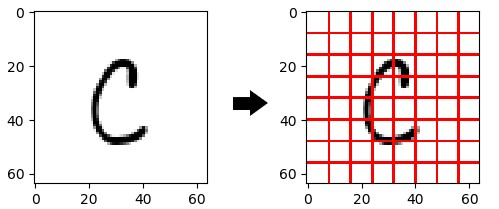
\includegraphics[height=6em]{img/textDetection/feature_zoning.jpg}
&
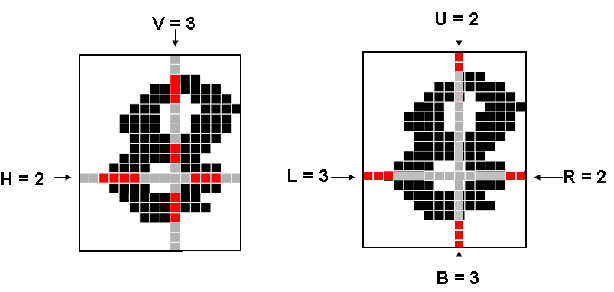
\includegraphics[height=6em]{img/textDetection/feature_crossing.png}
\end{tabular}
}
\caption{Example of two feature extraction techniques based on statistical representation (images by~\citet{statisticalFeatures}).}
\label{fig:featureExtractionStatistical}
\end{figure}

\begin{figure}[t]
\centering
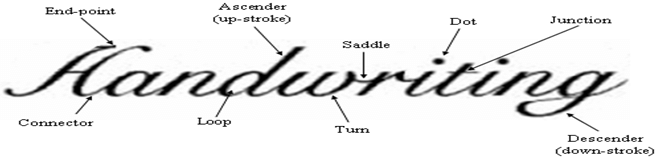
\includegraphics[width=0.8\linewidth]{img/textDetection/features_geometrical.png}
\caption{Example of several geometrical and topological features, as presented by~\citet{geometricalFeatures}.}
\label{fig:featureExtractionGeometrical}
\end{figure}

\subsection{Character classification}

Character classification is the process of obtaining a digital form of a character from its features. To classify the characters, OCR engines widely use the methodologies of pattern recognition, which assign an unknown sample into one of its predefined classes. These approaches are not necessarily independent of each other and OCR engines frequently combine subsets of them to achieve the most accurate results.

Classification is often approached by one of the following types of techniques:
\begin{itemize}
    \item Template matching
    \item Statistical techniques
    \item Techniques inspired by machine learning
\end{itemize}

In this section, we discuss their core principles.

The first mentioned approach to classification is by \emph{template matching}~\citep{templateMatching}, visualized in~\cref{fig:characterClassTemplate}. It is based on the existence of a database of predefined \emph{templates} --- multiple bitmaps containing characters of the alphabet. Improved version of this method have extended this database to include numbers and special characters. Once a character is detected, it is passed to the algorithm and for every existing template, its similarity ratio is calculated. The template with the greatest ratio is then assumed to be the recognized character. This method has various implementations depending on how the ratio is calculated --- for example, cross correlation, normalized correlation or euclidean formula can be used.

Although the implementation of this method is very simple, even small disfigurements and noise can greatly affect its efficiency. Also, in case of template matching, a feature extraction would be unnecessary as all templates must be created manually.

\begin{figure}[t]
    \noindent
	\makebox[\textwidth]{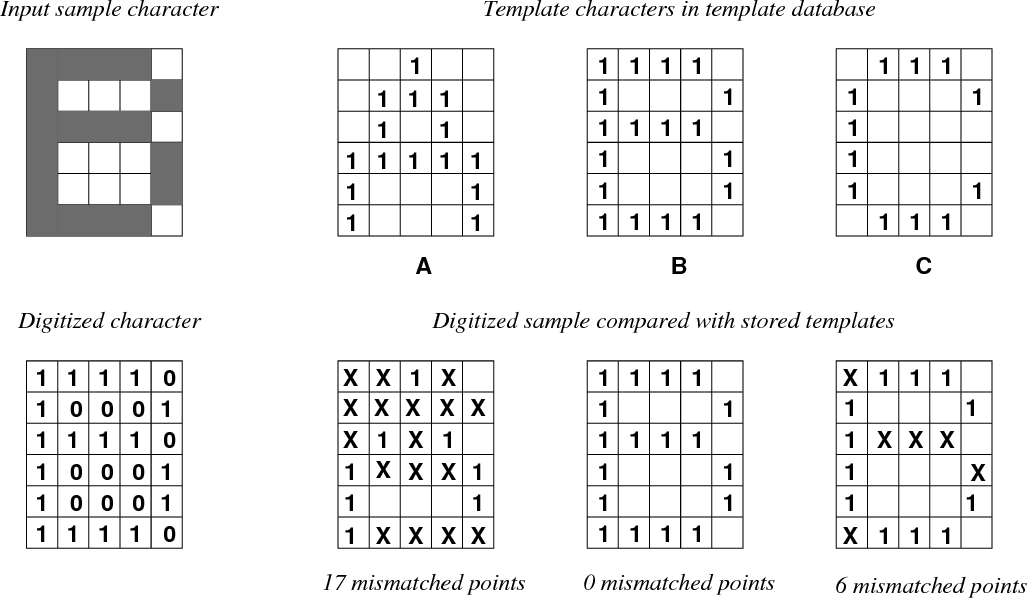
\includegraphics[width=30em]
	{img/characterClassification/templates.png}}
	\caption{Examples of template matching technique as described by~\citet{Ning1993AnIO}.}
	\label{fig:characterClassTemplate}
\end{figure}

The second approach mentioned was by using \emph{statistical techniques}~\citep{characterClassification}, like Bayes classifier, Hidden Markov Modeling or Nearest Neighbor. These methods are based on feature extraction for each character. To classify an unknown character, its extracted features are compared to the features of training data with the help of statistical decision functions. We show some of the possible extracted features for these methods in~\cref{fig:characterClassificationStatis}.

The problem with these methods is that they have no information about whole-part relations. Moreover, they greatly rely on the correctness and sufficiency of training data.

\begin{figure}[t]
\centering
{\sffamily
\begin{tabular}{ccc}
Existence and number & Number of & Number of \\
of end points & vertical lines & horizontal lines \\
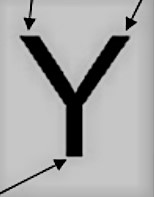
\includegraphics[height=10em]{img/characterClassification/statis_endPoint.jpg}
&
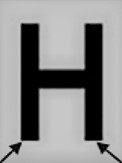
\includegraphics[height=10em]{img/characterClassification/statis_vertical.jpg}
&
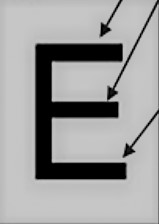
\includegraphics[height=10em]{img/characterClassification/statis_horizontal.jpg} \\
\end{tabular}
}
\caption{A few of the possible extracted features in statistical techniques~\citep{vithlani2015structural}.}
\label{fig:characterClassificationStatis}
\end{figure}

The last approach discussed are techniques inspired by machine learning~\citep{sebastiani2002machine}. These are based on neural networks, and their ability to ``learn'' and, over time, build a model of training data that is further used for categorizing their input. There is no requirement for manual categorization of individual data features, as the neural networks are capable of performing the feature extraction from training data on their own.

In the following list, we present an overview of some of the most popular machine learning algorithms, as described by~\citet{bhavsar2012comparative}:
\begin{itemize}
    \item \emph{KNN classification algorithm} --- the algorithm chooses K objects from the training data that are the most similar to the input image. After that, the image is assigned to the class most common among its K nearest neighbors, as shown in~\cref{fig:characterClassKNN}.
    \item \emph{Support vector machine algorithm} --- given a set of data, each marked as belonging to one of two categories, this algorithm builds a model based on complex mathematical functions that is capable of assigning a newly received data into one of the categories.
    \item \emph{Decision tree} --- builds a tree from top to bottom, with each node representing a characteristics feature and its children the values of the feature (e.g. number of horizontal lines).
\end{itemize}
Other machine learning algorithms are e.g. Naive Bayes~\cite{ng2002discriminative}, Logistic Regression~\cite{ng2002discriminative}, Random Forest~\cite{segal2004machine} etc.

\begin{figure}[t]
\centering
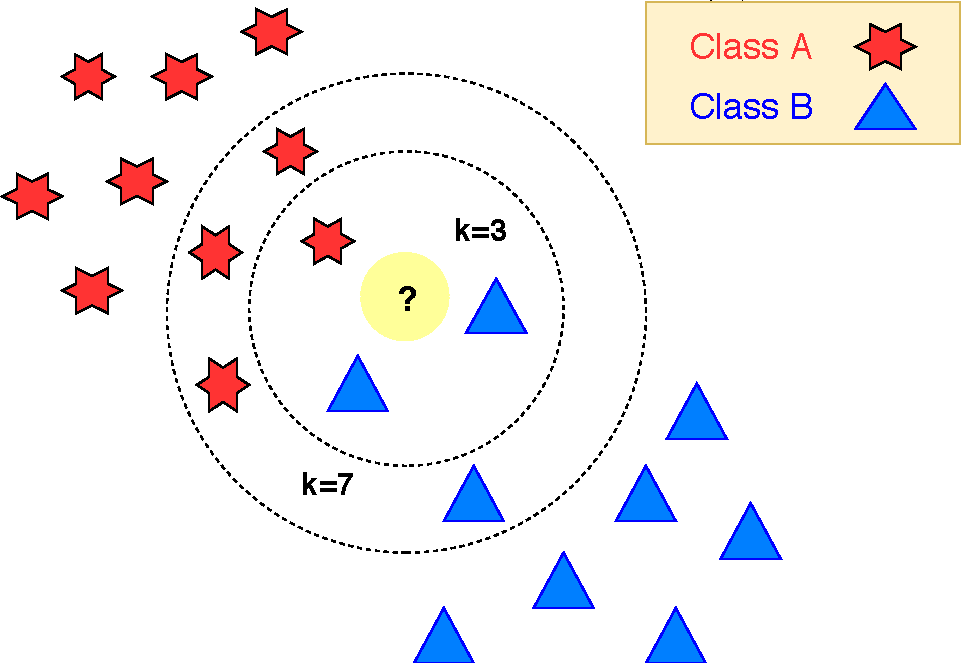
\includegraphics[width=0.7\linewidth]{img/characterClassification/knn.pdf}
\caption{KNN algorithm: with $k=3$, the algorithm will assign the new element to class B; with $k=7$ to class A.} \label{fig:characterClassKNN}
\end{figure}

Although our thesis is focused on the heuristic approach to OCR, neural networks are worth mentioning due to their growing usage in modern computer science.

\section{Available OCR software}

OCR engines greatly differ not only in the accuracy of their recognition, but also in the features that they provide. Although OCR engines focusing only on text recognition exist, most of the modern software also contains recognition of other document elements, like images, forms, tables and many more. Further differences include the presence of preprocessing options, support for various file extensions, recognition of different fonts, including handwritten documents, etc. Furthermore, there exist OCR engines specialized in processing only specific types of images, such as automatic number plate recognition engines or ticket validation engines.

In~\cref{tab:availableSoftware}, we overview the most popular and widely used free OCR engines. Commercial software used for the purposes of OCR, such as ABBYY FineReader~\cite{ABBYYSW}, ReadIris~\cite{ReadIris} and OmniPage~\cite{OmniPage}, also deserves a mention. However, although some of these engines produce overall better results than the free software, they are unusable for the purposes of this thesis.

\begin{table}[t]
{\small
\begin{tabular}{p{4.6em}p{2em}p{3em}p{4.8em}cc}
\toprule
\textbf{Name} & \textbf{Year} & \textbf{Code} & \textbf{Languages} & \textbf{Layout analysis} & \textbf{Neural nets}\\
\midrule
Tesseract & 1985 & C++, C & 100+ & \textbullet & \textbullet \\
Ocrad & 2003 & C++ & Latin alphabet &  \textbullet & -- \\
GOCR & 2000 & C & 20+ & -- & -- \\
CuneiForm & 1996 & C, C++ & 28 & -- & -- \\
OCRopus & 2007 & Python & Latin script & -- & \textbullet \\

\bottomrule
\end{tabular}
}
\caption{Overview of available OCR software}
\label{tab:availableSoftware}
\end{table}

\subsection{Tesseract}

Originally developed by Hewlett-Packard Company around 1990~\citep{TesseractGIT}, Tesseract is one of the most robust and accurate open-source OCR engines. In the beginning, Tesseract could only accept TIFF images containing simple one-column text in English language. Since then, it has undergone a lot of improvements and added many features. As of today, Tesseract supports the processing of multi-columned documents, claims to support over 100 languages (including right-to-left text such as Arabic or Hebrew), works on different input and output image formats (with the help of Leptonica library~\citep{LeptonicaLIB}) and is available for Windows, Linux and even Mac OS. In its latest version (4.0.0), Tesseract also added a new neural network (specifically a LSTM network) focused on line recognition. 

Tesseract does not have a GUI and works as a command line program. It is used mostly for development purposes and provides an OCR engine (libtesseract) that gives developers a chance to create their own applications using tesseract API. Also, Tesseract contains no preprocessing algorithms. It advises users to preprocess the input images themselves~\citep{TesseractQual}.

Based on our observation, Tesseract provides the most features and in general cases, provides the best accuracy of element recognition among all the other open-source OCR engines. Moreover, we found its documentation, information about individual functions and even examples of use cases well-organized and easy to understand.

This is the reason why we use the recognition and features of this engine in our implementation.

\subsubsection{Tesseract character recognition} \label{tesseractCharacterRecognition}

In this section, we present an overview of the way Tesseract detects symbols and so-called \emph{textlines}, which are logical rows consisting of character symbols. Thoroughly analyzed by~\citet{smith2007overview}, this algorithm has the following steps:

\begin{enumerate}
    \item \emph{Page segmentation}
    
    Already discussed in~\cref{sectionTessPageSegm}, the Tesseract page segmentation algorithm is first performed to provide us with text regions of roughly uniform text size.
    
    \item \emph{Line finding}
     
     Upon obtaining text regions, heuristics like height filter and median filter are used to estimate the height of characters and remove noise, punctuation and other obstacles. The filtered so-called \emph{blobs} are then merged into lines by their y-coordinate and position, with focus on slight possible skew inaccuracies.
     
     Once the blobs are assigned to lines, they are merged based on heuristic criterion.
     
     \item \emph{Baseline fitting}
    
    The next step is to find a baseline for each line, as shown in~\cref{fig:textRecTesseractBaseline}. These baselines are fitted using a quadratic spline, as curved baselines can also be present.
    
    \item \emph{Character chopping}
    
    Upon determining lines, Tesseract tries to chop the existing words into characters. This is done by a determined constant pitch when handling fixed-pitch text. In case of non-fixed-pitch text~(\cref{fig:textRecTesseractSpacing}), Tesseract tries to determine the size of a character by measuring the gaps between its baseline and upper boundary. However, in case of inaccurate assumptions, the decision can still be changed after word recognition.
    
    \item \emph{Word recognition in case of non-fixed-pitch text}
    
    This step proceeds to further chop blobs that might have produced unsatisfactory results in the last step. It does so by using various heuristics, and although its results are pretty satisfactory, this process often results in higher number of chops than required. Although an associator that already has knowledge of existing characters tries to resolve this issue, the occurrence of slight mistakes can not be excluded.
    
    \item \emph{Character classification}
    
    Earliest versions of Tesseract used a static character classifier based on topological features. However, this approach was not robust to damaged characters in real-life images. This was solved by extracting multiple small features of fixed length from the unknown and merging them to match more robust features of a character, as shown in~\cref{fig:textRecTesseractChars}.
    
    Classification itself is then performed by matching the characters to a training data set and outputting the character that has the greatest number of similar features (where the ``greatest number'' computation is based on heuristics).
    
\end{enumerate}

\begin{figure}[t]
\minipage{\textwidth}
    \centering
    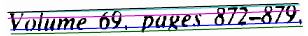
\includegraphics[width=0.7\linewidth]{img/textDetection/tesseractBaseline.png}
    \caption{An example of a fitted baseline (dark blue) along with helper lines used for baseline fitting and later, character chopping~\citep{smith2007overview}.}
    \label{fig:textRecTesseractBaseline}
\endminipage\\
\minipage{0.45\textwidth}
    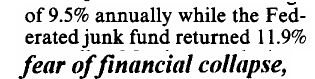
\includegraphics[width=\linewidth]{img/textDetection/tesseractSpacing.png}
    \caption{Non-fixed pitch text spacing issues~\citep{smith2007overview}.}
    \label{fig:textRecTesseractSpacing}
\endminipage\hfill
\minipage{0.45\textwidth}
    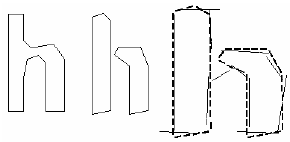
\includegraphics[width=\linewidth]{img/textDetection/tesseractCharacters.png}
    \caption{Left: original letter h; middle: broken character; right: merging of multiple smaller features~\citep{smith2007overview}.}
    \label{fig:textRecTesseractChars}
\endminipage
\end{figure}
